\documentclass{article}

\usepackage{lmodern}
\usepackage[T1]{fontenc}
\usepackage[spanish,activeacute]{babel}
\usepackage{mathtools}
\usepackage{graphicx}
\usepackage[utf8]{inputenc}


\title{TEMA 1 DESARROLLO DE SOFTWARE}
\author{Antonio Muñoz Cubero}
\date{1 de Ocutbre de 2020} 


\begin{document}
\maketitle
\pagenumbering{gobble}


Resumen del Tema 1 \textit{(Desarrollo de Software)} para la asignatura \textbf{Entornos de Desarrollo} en el 
\textit{I.E.S Francisco de los Rios} para el \textit{Grado Superior de Desarrollo de Aplicaciones Multiplataforma}.

\begin{figure}[b]
    
\includegraphics[width=1\linewidth]{cabecera_50_aniversario.png}
    \centering    
\end{figure}

\newpage

    \tableofcontents

\newpage
\pagenumbering{roman}

\section{Introducción}
\subsection{¿Qué es un Software?}

Conocemos como \textbf{\textit{Sofware}} al soporte lógico de un sistema infomático, que comprende el cunjunto de los
componentes lógicos necesarios que hacen posible la realización de tareas específicas, en contraposición
los componentes físicos que son nombrados \textit{"Hardware"}.\\

La interación entre el \textbf{\textit{Sofware}} y el \textit{Hardware} hace operativo a un ordenador o cualquier otro 
dispositivo, es decir, el \textbf{\textit{Sofware}} envía instrucciones que el \textit{Hardware} ejecuta, haciendo posible 
el correcto funcionamiento de la máquina utilizada.\\

El \textbf{\textit{Sofware}}, en su mayoria, está escrito en lenguajes de programación de alto nivel, ya que son más fáciles
y eficientes para que los programadores los usen, ya que son los más cercanos al lenguaje natural respecto al lenguaje máquina.
Los lenguajes de alto nivel se traducen a lenguaje máquina para que esta la interprete y realice las acciones descritas en el código
\textbf{\textit{Sofware}} de alto nivel, usando bien un compilador o un interprete (algunos lenguajes necesitan de un híbrido de ambos).

\section{Ciclo de vida Sofware}
Un proceso de software es el conjunto de actividades necesarias para transformar los requisitos de un usuario en un sistema software. 
Cuando implica la construcción de un producto, se suele llamar ciclo de vida e incluye el periodo de tiempo comprendido desde la definición 
de los requisitos hasta el fin de su uso. El ciclo de vida presenta unos procesos primarios, como se reflejan en la siguiente imagen.
\\

\begin{figure}[b]
   
    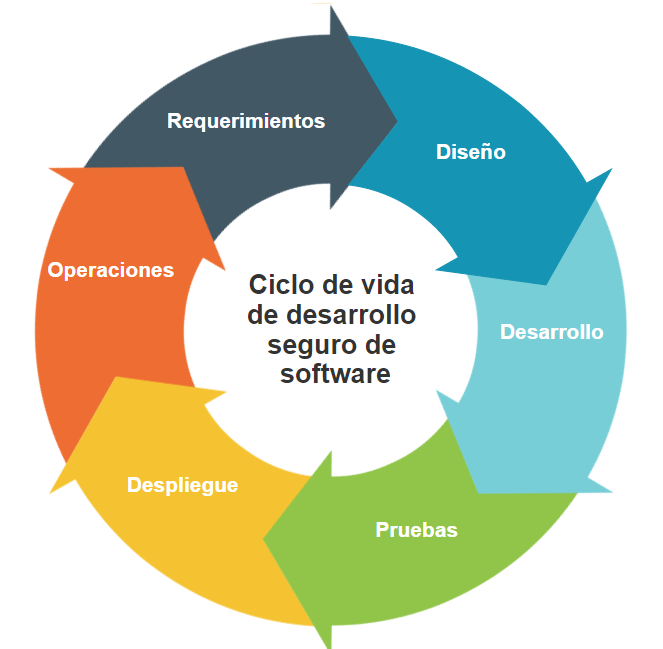
\includegraphics[scale=0.22]{Software-Development-Life-Cycle.png}
    \centering
    
\end{figure}

\newpage
\section{Fases del Desarrollo Software}
La aplicación de procesos, tanto en el desarrollo como en el posterior mantenimiento y operación del software siguen unos “patrones fijos” 
que configuran el esquema de mapa de situación, relación y continuidad entre los diferentes procesos, actividades y tareas. La etapa de 
desarrollo da paso al ciclo de vida del sistema y en las diferentes etapas del ciclo de vida pueden intervenir modificadores.
\\
Existen varios modelos de ciclos de desarrollo, estos aplican distintas metodologías que se adaptan mejor al desarrollo específico de un tipo 
de Software, por consiguiente, explicaremos los diferentes ciclos de desarrollo.
\\
\subsection{Modelo Secuencial}
Este modelo refleja un desarrollo marcado por la sucesión escalonada de las etapas que lo componen: \textbf{requisitos – diseño – codificación – pruebas – integración.}
Cada etapa da lugar a la siguiente sólo cuando termina, por lo que resulta muy rígido y genera problemas. Resulta apropiado para desarrollar versiones de sistemas 
ya veteranos en los que el desconocimiento de las necesidades de usuarios o del entorno no plantea riesgos y para sistemas pequeños.
\\
\\
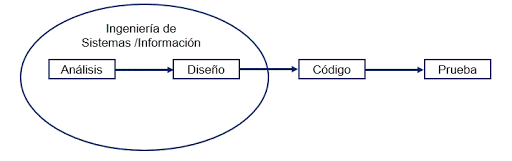
\includegraphics[width=1\linewidth]{secuencial_1.png}
\\
\\
En numerosos documentos, toman el modelo secuencial como símil del modelo en cascada, pero este último a continuación podremos proceder a visualizar y comprender
las diferencias y similitudes que mantiene con el sistema secuencial, ambos son modelos de desarrollo software no ágiles, estos los veremos mas adelante puesto que 
marcan un gran avance en la produccion y calidad del Software moderno.

\newpage
\subsection{Modelo en Cascada}
Modelo prácticamente idéntico al secuencial, \textbf{añade la posibilidad de retornar desde una fase hacia las anteriores con la información generada al avanzar el desarrollo.} 
Este modelo reconoce la importancia de disponer de unos requisitos y un diseño previo antes de comenzar con la codificación del sistema. Resulta apropiado para los mismos 
casos que el secuencial. Un ejemplo de metodología de desarrollo en cascada es la siguiente imagen:
\\
\\
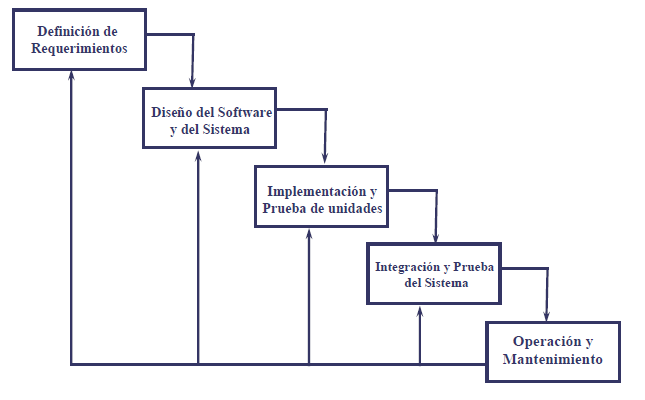
\includegraphics[width=1\linewidth]{cascada.png}
\\
\\
De esta forma, cualquier error de diseño detectado en la etapa de prueba conduce necesariamente al rediseño y nueva programación del código afectado, aumentando los costos del desarrollo. 
La palabra cascada sugiere, mediante la metáfora de la fuerza de la gravedad, el esfuerzo necesario para introducir un cambio en las fases más avanzadas de un proyecto. 
Si bien ha sido ampliamente criticado desde el ámbito académico y la industria, sigue siendo el paradigma más seguido al día de hoy.

\newpage
\subsection{Modelo en Espiral}
Este diseño presenta un desarrollo evolutivo, además de introducir el análisis de riesgo para guiar la evolución del proceso de desarrollo.
El ciclo de iteración de este modelo se convierte en una espiral, que al representarse sobre ejes cartesianos muestra en cada cuadrante una 
clase particular de actividad: planificación, análisis de riesgo, ingeniería y evaluación. La dimensión angular representa el avance relativo 
en el desarrollo de las actividades de cada cuadrante. En cada ciclo de la espiral se realiza una parte del desarrollo total, a través de los 
cuatro tipos de actividades, como vemos en la siguiente imagen:
\\
\\
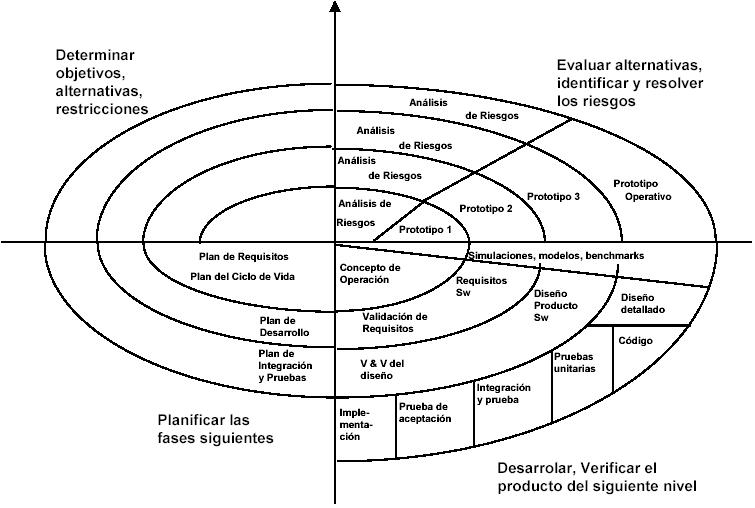
\includegraphics[width=1\linewidth]{espriral.png}
\\
\\
En la \textbf{planificación} se establece el contexto del desarrollo y se decide qué parte del mismo se abordará en el ciclo siguiente.
En \textbf{análisis de riesgo} se evalúan las alternativas posibles para la ejecución de la siguiente parte del desarrollo, seleccionando la más ventajosa y previendo los riesgos posibles.
Las \textbf{actividades de ingeniería} corresponden a las indicadas en los modelos lineales: análisis, diseño, codificación, etc.
Las \textbf{actividades de evaluación} analizan los resultados de la fase de ingeniería, tomando el resultado de la evaluación como punto de partida para el análisis de la siguiente fase.

\newpage
\subsection{Metodologías Ágiles}
Por definición, las \textbf{metodologías ágiles} son aquellas que permiten adaptar la forma de trabajo a las condiciones del proyecto, consiguiendo flexibilidad e inmediatez en la respuesta para 
amoldar el proyecto y su desarrollo a las circunstancias específicas del entorno. En esencia, las empresas que apuestan por esta metodología \textbf{\textit{consiguen gestionar sus proyectos de forma 
flexible, autónoma y eficaz reduciendo los costes e incrementando su productividad.}}
\\
\\
\begin{figure}[h]
    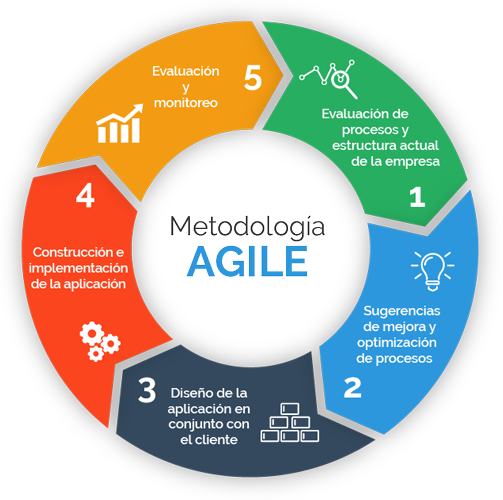
\includegraphics[scale=0.35]{Metodologia-agile_hd.png}
    \centering
\end{figure}
\\
\\
La definición moderna de desarrollo ágil de software evolucionó a mediados de la década de 1990 como parte de una reacción contra los métodos de "peso pesado", muy estructurados y estrictos, 
extraídos del modelo de desarrollo en cascada. El proceso originado del uso del modelo en cascada era visto como burocrático, lento, degradante e inconsistente con las formas de desarrollo de 
software que realmente realizaban un trabajo eficiente. 
\\
En el año 2001, miembros prominentes de la comunidad se reunieron en Snowbird, Utah, y adoptaron el nombre de \textbf{"métodos ágiles"}. Poco después, algunas de estas personas formaron la "alianza ágil", 
una organización sin fines de lucro que promueve el desarrollo ágil de aplicaciones. Muchos métodos similares al ágil fueron creados antes del 2000. Entre los más notables se encuentran: \textit{Scrum} (1986), 
\textit{Crystal Clear} (transparente como el cristal), \textit{programación extrema} (en inglés eXtreme Programming o XP, 1996).

\newpage
\subsubsection{Scrum}
Scrum es un proceso de gestión que reduce la complejidad en el desarrollo de productos para satisfacer las necesidades de los clientes. La gerencia y los equipos de Scrum trabajan juntos alrededor de requisitos 
y tecnologías para entregar productos funcionando de manera incremental usando el empirismo. Scrum es un marco de trabajo simple que promueve la colaboración en los equipos para lograr desarrollar productos complejos. 
\begin{figure}[h]
    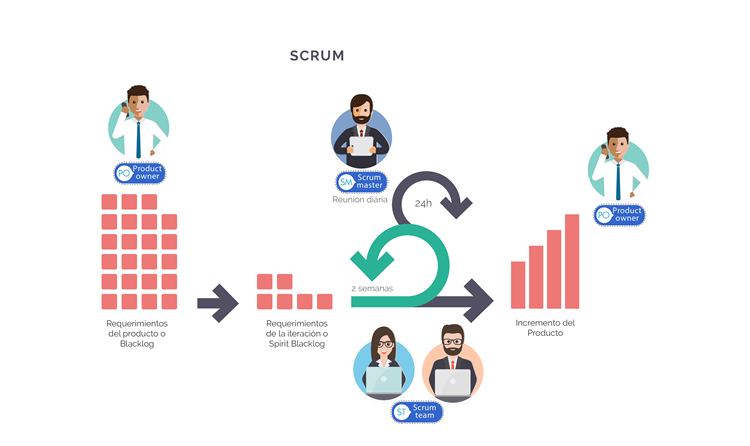
\includegraphics[width=1\linewidth]{scrum_1.png}
\end{figure}
\\
En Scrum no se realiza una entrega final del proyecto sino que se van haciendo de forma regular entregas parciales, de forma que esto es lo que más beneficia al receptor del proyecto.  Por ello, Scrum está especialmente 
indicado para entornos complejos, donde los cambios se producen como mucha frecuencia y sobre la marcha y donde la rapidez, la flexibilidad, la adaptabilidad y la competencia juegan un papel fundamental. El marco de scrum 
lo forman los siguientes componentes:
El marco de scrum técnico está formado por:

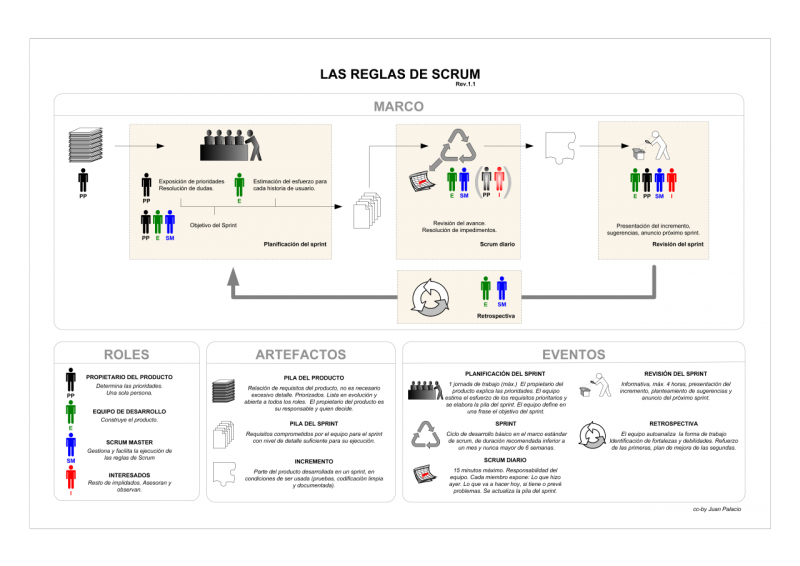
\includegraphics[scale=0.25]{800px-Marco_estandar_scrum.png}

\textbf{Roles:}
\begin{itemize}
    \item El equipo scrum.
    \item El dueño del producto.
    \item El Scrum Master.
\end{itemize}

\textbf{Artefactos:}
\begin{itemize}
    \item Pila del producto.
    \item Pila del sprint.
    \item incremento.
\end{itemize}

\textbf{Eventos:}
\begin{itemize}
    \item Sprint.
    \item Reunión de planificación del sprint.
    \item Scrum diario.
    \item Revisión del sprint.
    \item Retrospectiva del sprint.
\end{itemize}

\newpage
\section{Concepto de Programa Informático}
Programa es un concepto con numerosas acepciones. Puede tratarse de una planificación, un temario, un cronograma, una unidad temática o una emisión de radio o televisión, por citar algunas posibilidades.
\\
Cuando hablamos específicamente de programa en informática, estamos haciendo referencia a un software. \textbf{Se trata de aplicaciones y recursos que permiten desarrollar diferentes tareas en una computadora (ordenador), 
un teléfono u otros equipos tecnológicos}. Para desarrollar un programa informático, se necesita apelar a los lenguajes de programación que posibilitan el control de las máquinas. A través de diversas reglas semánticas 
y sintácticas, estos lenguajes especifican los datos que transmite el software y que tendrá que operar la computadora. Además del citado lenguaje, también es fundamental dentro de cualquier programa en informática o 
programa informático tanto el archivo fuente como el editor de vínculos, el archivo ejecutable, el compilador o el archivo objeto. Existen diferentes tipos de programas en informática. El software de base, por ejemplo, 
es aquel que le brinda a la persona el control sobre los elementos físicos de la computadora, que se conocen como hardware. Dentro del software de base puede nombrarse a los sistemas operativos, como Windows o Linux.
\\
\\
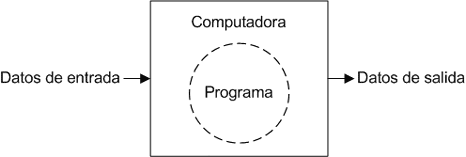
\includegraphics[width=1\linewidth]{programa.png}
\\
\\

\newpage
\section{Obtención del Código de Ejecución}
Podemos empezar este punto con la idea de que los programas informáticos funcionan, o bien, compilando el código fuente de un lentguaje de alto nivel, esto es necesario en lenguajes compilados como pueden ser \textit{C, C++, etc},
sin embargo, no todos los lenguajes son compilados, hay lenguajes que son \textbf{interpretados} como pueden ser \textit{Java, JavaScript, Python, etc}. Teniendo esto en cuenta vamos a definir que es compilar para despues explicar 
que es interpretar y mostraremos sus diferencias.
\subsection{Compiladores}
Un compilador es un pequeño programa informático, que \textbf{se encarga de traducir (compilar) el código fuente de cualquier aplicación que se esté desarrollando}. En pocas palabras, es un software que se encarga de traducir el programa 
hecho en lenguaje de programación, a un lenguaje de máquina que pueda ser comprendido por el equipo y pueda ser procesado o ejecutado por este. Un concepto un poco más elaborado es el siguiente: Un compilador es un programa que 
convierte o traduce el código fuente de un programa hecho en lenguaje de alto nivel, a un lenguaje de bajo nivel (lenguaje de máquina).
\\
\\
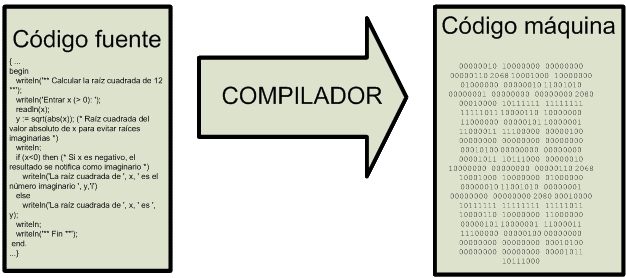
\includegraphics[width=1\linewidth]{compilador.png}

\newpage
\subsection{Interprete}
Un intérprete \textbf{es un software que recibe un programa en lenguaje de alto nivel, lo analiza y lo ejecuta}. Para analizar el programa completo, va traduciendo sentencias de código y ejecutándolas si están bien, así hasta completar el programa origen.
Los intérpretes informáticos, al contrario que los compiladores, no generan un fichero ejecutable u otro programa equivalente en otro lenguaje, por lo que cada vez que se ejecuta el programa original debe pasar por la fase de análisis. Esto hace 
de \textbf{los intérpretes más lentos que los compiladores}, donde las fases de análisis y ejecución son independientes, por lo que solo se compila una vez y se ejecuta cuantas veces se quiera. Comparando su actuación con la de un ser humano, un compilador 
equivale a un traductor profesional que, a partir de un texto, prepara otro independiente traducido a otra lengua, mientras que un intérprete corresponde al intérprete humano, que traduce de viva voz las palabras que oye, sin dejar constancia por escrito. 
\\
\\
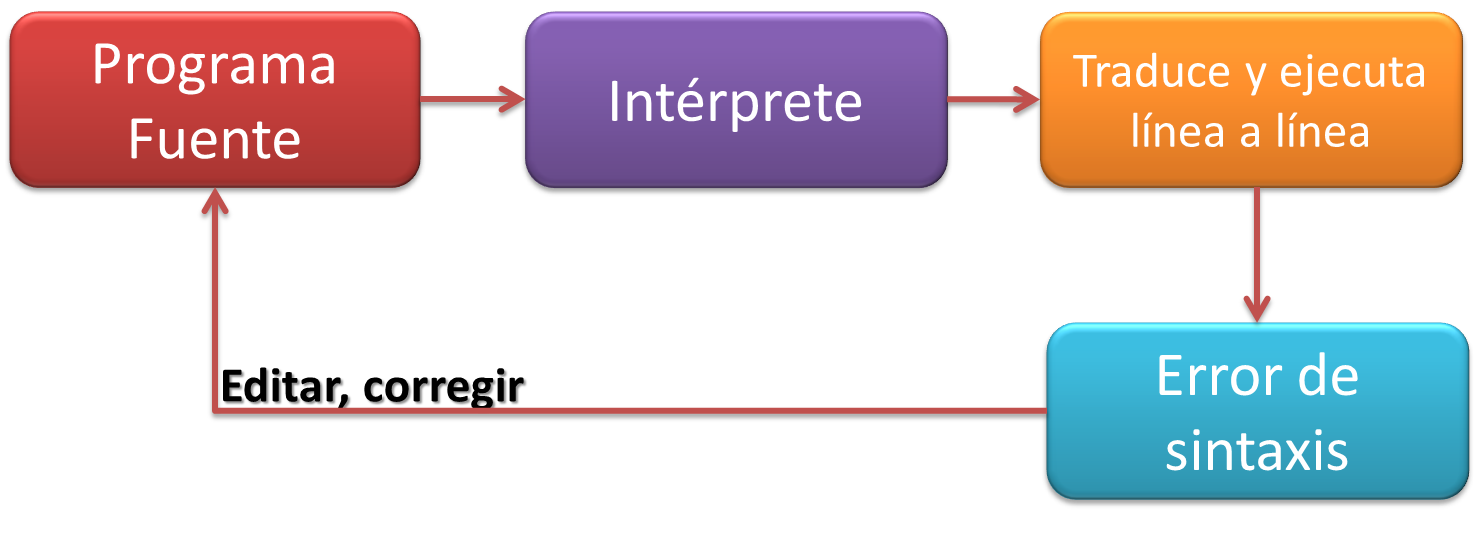
\includegraphics[width=1\linewidth]{Interprete.png}

\end{document}



